\documentclass[10pt, letterpaper]{article}
\usepackage[a4paper, total={18cm, 26cm}]{geometry}
\usepackage{graphicx}
\usepackage{amsmath}
\usepackage{amssymb}
\usepackage{booktabs}
\usepackage{nicefrac}
\usepackage{multicol}
\usepackage{lipsum}% http://ctan.org/pkg/lipsum
\usepackage{algorithm}
\usepackage[algo2e]{algorithm2e} 
\usepackage{multirow}
\usepackage[pagebackref,breaklinks,colorlinks]{hyperref}

% Support for easy cross-referencing
\usepackage[capitalize]{cleveref}
\crefname{section}{Sec.}{Secs.}
\Crefname{section}{Section}{Sections}
\Crefname{table}{Table}{Tables}
\crefname{table}{Tab.}{Tabs.}

\begin{document}
\author{
zain bin sumait}
\nocite{*}

\begin{figure}[thpb]
    \centering
    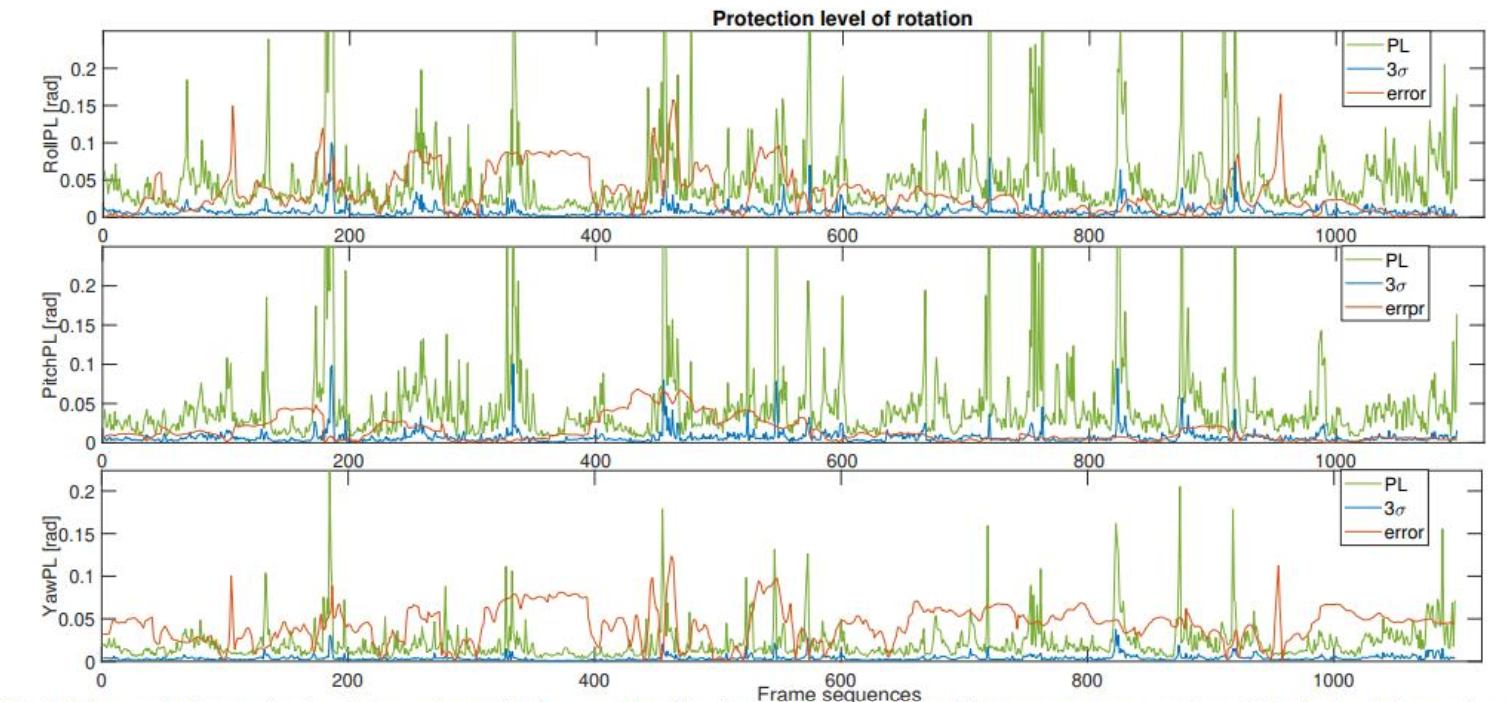
\includegraphics[width=\textwidth]{images/frame_se1.png}
    \caption{The trend of protection level}
    \label{fig:Frame_sequence}
\end{figure}
%% Here goes your code
\begin{multicols*}{2}
4) The Discussion of PL


Ideally, the PL should be able to cover the error, but the facts
contradict this. Based on the derivation of PL in Section IV-C,
the calculation of PL is affected by bias-induced error resulting
from outliers and noise-induced error because of observation
noises. Firstly, the number of outliers existing in the current
observations after passing the Chi-square test is unknown.
Secondly, the noise covariance matrix of the visual
measurements cannot be obtained exactly which is given
empirically in this paper. All these uncertainties are factors that
can affect the performance of PL estimation.


To gain more insight into PL, we evaluate the bound rate of
PL and 3$\sigma$ under different assumptions with multiple outliers
and noise covariances in Table II. From Tables II, it can be seen
that increasing the number of outliers can improve the bound
rate of PL, but when the number of outliers is set to 3, it will
not change, indicating that the largest number of outliers in all
sequences is 2. In Table III, the measurement noise of the line
feature is set to 3, 5, and 7 pixels, respectively. In practice, the
measurement noise of a single pixel point feature is usually set
between 1-3 pixels [56]. Since this paper uses line features, the
detection of lines will introduce more errors than point features.
Also, the 3D line features extracted from the point cloud map
could impose observation error, so the covariance assumption
is amplified here. Similarly, the same assumption is used for the
Chi-squared test above. It can be seen from Table III that as the
covariance increases, the rate rises, which means that PL is
getting larger. In summary, more outliers and larger covariance
increase PL, which is consistent with the definition of PL for
quantifying safety, where larger error noise could lead to larger
PL.

A specific analysis is done for the case of abnormal PL where
the PL cannot reliably bound the localization error. Based on
the experiments above, it is known that PL is influenced by the
quality of observations. Moreover, the distribution of the line features utilized for the localization is the other sources
affecting the PL estimation. It is expected that the features are
uniformly distributed horizontally and vertically which could
introduce optimal constraints. However, the case could occur
where the features flock together which can lead to the
degeneration of the state estimation [57]. To quantify the
impacts of the feature distribution on the localization
performance, the inverse condition number (ICN) is introduced
in [57]. In particular, the ICN is determined by the inverse of
the ratio between the minimum and maximum eigenvalues of
$J^T J$ ,where, the J denotes the Jacobian matrix of the visual line
constraint which is rigorously derived in the appendix of this
paper.
\begin{figure}[H]
    \centering
    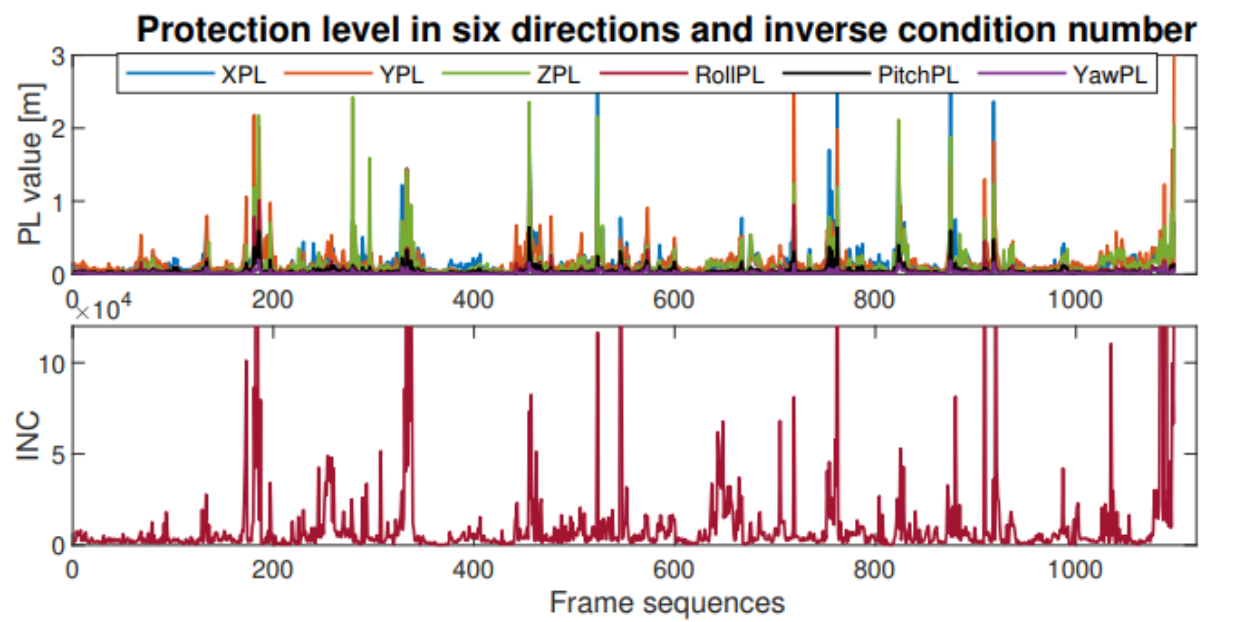
\includegraphics[width=\columnwidth]{images/frame_se2.png}
    \caption{The inverse condition number (ICN) and comparison of protection level, 3$\sigma$, and error in three translation }
    \label{fig:Frame_sequence2}
\end{figure}
\cref{fig:Frame_sequence2} displays the ICN and PL in three directions. As seen
from the figure that PL has a highly consistent trend with ICN
at the abnormal mutation, which indicates that these frames
have ill-conditional constraints and feature degeneration. Based
on this discovery, we can conclude that feature degeneration
largely causes exceptional maxima peak in PL. On the other
hand, we could utilize PL to remind the feature degeneration
phenomenon during state estimation to avoid serious
optimization failures. \cref{fig:table_ab1} shows two typical feature
degeneration scenarios. It is clear that most of the features in
images are parallel, which makes the constraint with its vertical
direction very weak, resulting in an ill-condition case.

\begin{figure}[H]
    \centering
    \begin{tabular}{cc}{}
    %\hline
        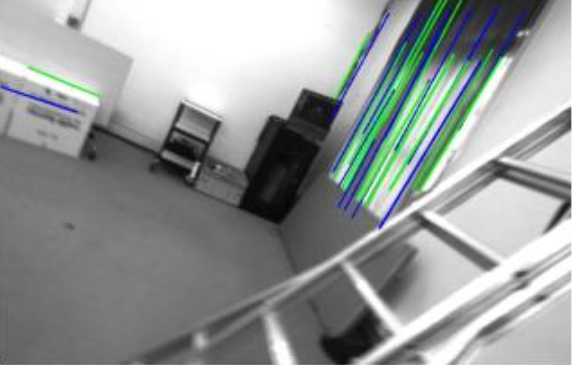
\includegraphics[width=0.48\columnwidth]{images/a1.png}&
        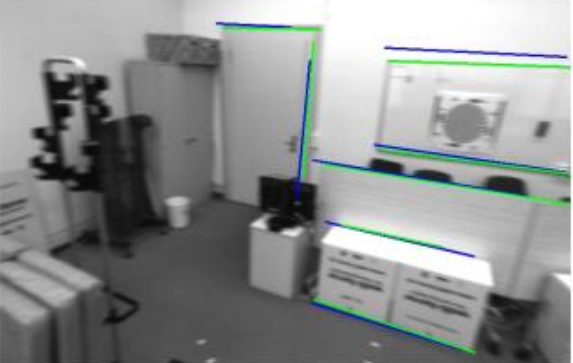
\includegraphics[width=0.48\columnwidth]{images/b1.png}\\
         (a)  & (b) \\
         
    \end{tabular}
    \caption{Two examples of the features degeneration.}
    \label{fig:table_ab1}
\end{figure}

\begin{figure}[H]
    \centering
    \begin{tabular}{cc}{}
    %\hline
        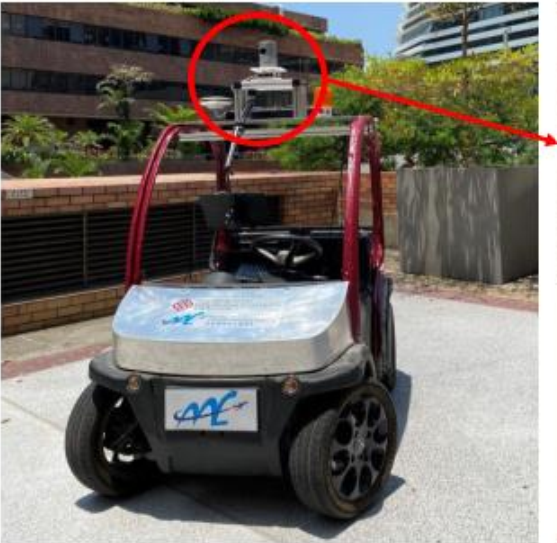
\includegraphics[width=0.48\columnwidth]{images/a2.png}&
        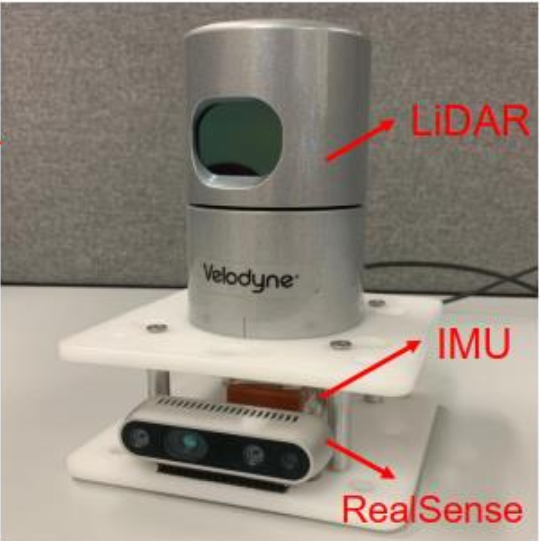
\includegraphics[width=0.48\columnwidth]{images/b2.png}\\
         (a)  & (b) \\
         
    \end{tabular}
    \caption{Two examples of the features degeneration.}
    \label{fig:table_ab2}
\end{figure}

B. UGV Outdoor Experiment
\begin{enumerate}%[label=\arabic*]
                \item  Experiment Setup

                
The UGV platform used in this experiment is shown in \cref{fig:table_ab2} (a), and (b) is the sensor suite, which contains a LiDAR
(HDL 32E Velodyne, 10 Hz), an IMU (Xsens Mti 10, 200 Hz),
and a RealSense camera (D435i, 30 Hz). The dataset is
collected by driving around a square on the Hong Kong
Polytechnic University (PolyU) campus (\cref{fig:table_ab3} (b)). The total
path length is 295.5 m. The IMU data and images captured by
RealSense are the input of VINS. The data from LiDAR and
IMU are processed by LIO\_SAM implementation [58], and
used to build a prior point cloud map shown in \cref{fig:table_ab3} (a), the
origin of this 3D map is defined at the starting position of the
IMU. The trajectory estimated by LIO\_SAM is regarded as the
ground truth of localization. With the help of the LiDAR loop
closure, centimeter-level accuracy can be obtained from the
LIO\_SAM in the evaluated scene. Accordingly, similar
evaluation criteria and comparisons with UAV experiment are
adopted in this section.
                \item System Evaluation


                Table IV lists the RMSE of ATE comparison results of the
proposed method with VINS and benchmark, which can be seen
that our algorithm can also improve the localization accuracy in
the outdoor environment using UGV. \cref{fig:Frame_sequence3} presents the
estimation errors of translation and rotation, it is clear our
algorithm is able to reduce the drift problem of VINS to some
extent, which is evident in the z and yaw motions, while the
errors in other directions can be offset periodically because the
UGV trajectory is a constantly repeating circular motion.
However, as the path keeps getting longer and the VINS drift
increases, the effectiveness of our algorithm for removing the
cumulative error gradually diminishes (see \cref{fig:Frame_sequence3}) due to the
fact that the proposed method uses the output of VINS as the
initial guess.

\begin{figure}[H]
    \centering
    \begin{tabular}{cc}{}
    %\hline
        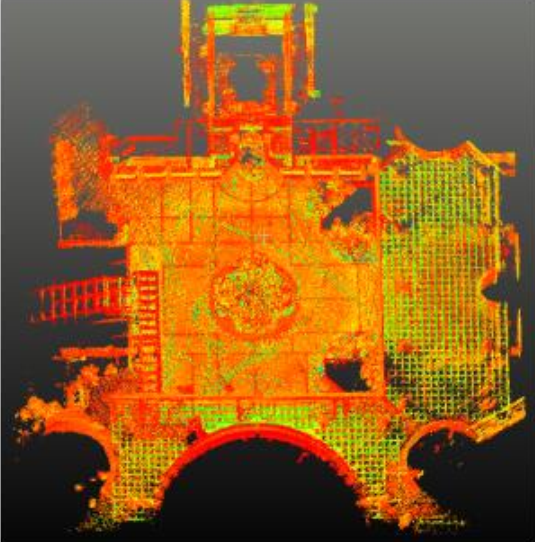
\includegraphics[width=0.48\columnwidth]{images/a3.png}&
        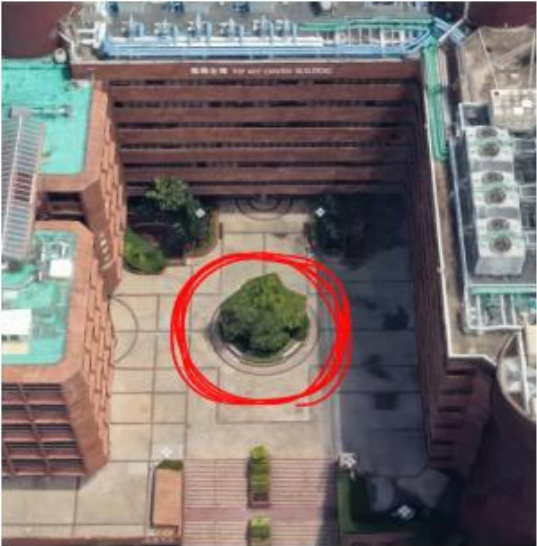
\includegraphics[width=0.48\columnwidth]{images/b3.png}\\
         (a)  & (b) \\
         
    \end{tabular}
    \caption{Two examples of the features degeneration.}
    \label{fig:table_ab3}
\end{figure}

\begin{table}[H] %table* pour la metre dans le meme format que la page 
    \centering
    \begin{tabular}{ccccc}{5cm}
    \hline
        Sequence & VINS  & Benchmark & PPL & PPL-OR\\
         & [6] & [30] & [ours] & [ours]\\
    \hline
     Poly Campus & 1.688 & 2.191 & 1.607 & \textbf{1.602} \\
    \hline
    \end{tabular}
    \caption{ Cumulative errors and the proportion of occupied cells for each combination}
    \label{tab:my_table}
\end{table}

\begin{figure}[H]
    \centering
    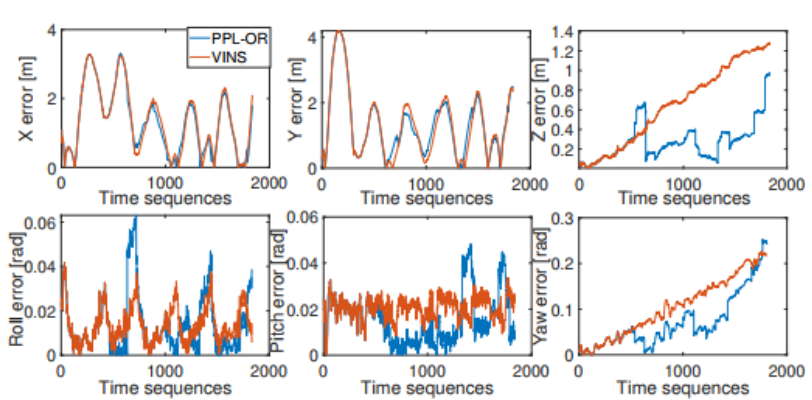
\includegraphics[width=\columnwidth]{images/seq3.png}
    \caption{The position and orientation error  }
    \label{fig:Frame_sequence3}
\end{figure}
\end{enumerate}

\begin{table}[H] %table* pour la metre dans le meme format que la page 
    \centering
    \begin{tabular}{ccccccc}
    \hline
        Num. & $x$  & $y$ & $z$ & $roll$ & $pitch$ & $yaw$\\
        1 & 83.1(\%) &66.2(\%) & 50.8(\%) & 64.6(\%) & 53.9(\%) & 5.13(\%)\\
        1 & 83.1(\%) &66.2(\%) & 50.8(\%) & 64.6(\%) & 53.9(\%) & 5.13(\%)\\
        1 & 83.1(\%) &66.2(\%) & 50.8(\%) & 64.6(\%) & 53.9(\%) & 5.13(\%)\\
    \hline
    \end{tabular}
    \caption{ Cumulative errors and the proportion of occupied cells for each combination}
    \label{tab:table2}
\end{table}

Based on the discussion of PL in the previous subsection, the
safety quantification of UGV is verified by adjusting the
number of outliers and the covariance of measurements. By
fixing the covariance to $7-pixel^2$, the relationship between the
bound rate of PL and the number of outliers is shown in Table
V. It is clear that the number of residual outliers in the UGV
dataset is two, which is the same as the UAV experiment. Next,



{\small
\bibliographystyle{IEEEtran}
\bibliography{references}
}
\end{multicols*}
\end{document}